\chapter{Electromagnetic Field Quantization and Electromagnetic Worldline Path Integrals}

\label{ch:EM_quantization}

This chapter develops the worldline path integrals for electromagnetism with a space-dependent
dielectric function, paralleling the treatment of the Dirichlet scalar worldline method in Ch.~\ref{ch:introduction}.  
First, we will review prior work on quantizing the EM field inside media.
Following that, we will review classical EM field theory and quantize the EM field.
The partition function for the EM field will be developed as a path integral in terms of the scalar and vector potentials.
However, the resulting worldline path integrals for the full set of potentials pose a number of challenges.
As a result, we turn our attention to developing scalar models that better capture the features
of electromagnetism.  In fact, in planar geometries, the scalar models correspond to 
the amplitudes of the two transverse modes.  
% Then we introduce the classical field theory for the EM field in both Lagrangian and 
% Hamiltonian forms.  We quantize the theory, and then develop the partition function.
%The partition function can be converted to a Euclidean path integral, which still has a residual gauge-freedom.
%The gauge freedom is removed via Faddeev-Popov gauge fixing, with a space-dependent gauge. 
% We then develop the worldline path integral for the full gauge theory, and comment on the resulting
% structure.
% In the search for a more tractable model system, we will show that in planar geometries the 
% EM field can be split into two non-interacting scalar fields.
We will then develop the worldline path integrals for those scalar fields, which will form
the basis for our analytical and numerical work in Chapters~\ref{ch:analytical} and \ref{ch:numerical}.  

\section{Approaches to Quantizing Electromagnetism in Media}

The quantization of the EM field inside dielectric media provides a number of challenges 
beyond quantization in vacuum~\cite{Huttner1992,Dung1998,Bechler1999,Bordag1998,Rahi2009,Reid2013}.  
 First, in Casimir problems the dielectric varies spatially.  The usual procedure for
quantizing the EM field decomposes the field into a set of normal modes, and quantizes their amplitudes.
  While it is possible to write down the wave equations for the modes, and quantize the amplitudes
 in analogy with free space~\cite{Glauber1991}, a full development of this method still requires finding those mode functions.
 Ideally, the procedure used in quantizing the field would not require solving for the mode functions in
general geometries, nor would it be adapted to any particular geometry.   

Second, the dielectric complicates the choice of gauge-fixing.  
In brief, EM has a gauge symmetry, or redundant degrees of freedom, which must be 
excluded from the quantization procedure.  
The gauge symmetry can be removed by imposing a gauge condition on the fields.
  In free space this is typically done by fixing Coulomb or Lorenz gauge, which 
decouple the radiative and static electromagnetic problems, or maintain relativistic invariance, respectively.
However inside a dielectric (starting at the level of macroscopic fields) the usual gauge-fixings lose these nice
features, and must be replaced by a dielectric-dependent condition.  
This issue will be discussed further in Sec.~\ref{sec:gauge_fixing}.

Third, since the dielectric has some frequency response or dispersion, the Kramers-Kr\"onig relations 
require that there is also loss or dissipation.  
In  quantum optics, dissipation is usually handled by coupling the system to a bath, and then
integrating or tracing out the bath degrees of freedom.\footnote{If damping is added to the system in an ad hoc
manner, the canonical commutation relations between operators would decay away.  Adding the bath
is necessary to preserve the commutation relations for the system operators.  As a result, dissipation in quantum systems 
is attended by noise, either as decoherence terms in the master equation or as noise terms in the Langevin equations for the operators~\cite{GardinerZoller2004}}.
The light field is linearly coupled to the dielectric medium, which is modeled
as a bath of harmonic oscillators~\cite{Huttner1992,Dung1998,Bechler1999}.
The dielectric medium is in turn coupled to a bath of harmonic oscillators, which provides the damping.
Integrating out the bath degrees of freedom yields the required dispersion and dissipation for the medium, 
while integrating out the medium's degrees of freedom yields a frequency dependent dielectric constant $\epsilon(\omega)$.
Huttner and Barnett were the first to use this harmonic model to quantize the EM field in media. Their
work directly diagonalized the whole system of fields and bath in terms of the modes of 
a single combined harmonic oscillator~\cite{Huttner1992}.
Another approach to the same problem directly couples the medium to white noise sources to represent the fluctuations 
inside the medium that lead to dissipation~\cite{Scheel1998,Dung1998,Tip2001}.
Bechler carried out path integral quantization for a harmonic medium 
including dispersion, and shown agreement with previous results in terms 
of noise operators and commutators for the fields~\cite{Bechler1999,Bechler2006}.  
It is not strictly necessary to assume that the fields are directly coupled to harmonic oscillators. 
The dielectric function can be understood in terms of the linear response of the underlying 
medium (which might not be harmonic) to the EM field~\cite{Altland2011}.  
This was used by Rahi\etal to motivate the effective Lagrangian description in terms of macroscopic field in their 
work on the scattering method~\cite{Rahi2009}.  
More recently Philbin carried out a full canonical quantization of EM in media, without explicitly 
assuming a harmonic medium~\cite{Philbin2010}.

%It is not strictly necessary to start at the microscopic level of the interaction of the 
% The field action is quadratic in the fields, and there are only linear couplings between other
% harmonic fields, the resulting path integrals are also Gaussians.  Such Gaussian path integrals 
% are straightforward to evaluate (certainly in comparison with the nonlinear field theories condensed
% in condensed matter and high energy physics where perturbation theory is the only recourse.)
% The primary results in Bechler's work were finding the form of the field propagator, and showing consistency with the 
% other approaches by Huttner and Barnett~\cite{Huttner1992} and Langevin equations by Dung\etal\cite{Dung1998},
%  rather than new computations exploiting the propagator. 
%  The results were all framed in terms of the 
% Fourier decompositions of the fields in terms of wavenumber, which is unsuitable for a worldline procedure.

Focusing on Casimir physics, in modern treatments the EM field has been quantized via path integration.
Reid\etal quantize the EM field, under the assumption of piecewise constant dielectric media, where the EM
boundary conditions are explicitly enforced at the interfaces~\cite{Reid2013}.
Enforcing those boundary conditions allows the remaining computations to proceed
as if the media were homogeneous and filled all of space, based on a version of Green's theorem~\cite{Emig2004}.
Fixing the boundary conditions also simplifies the algebra, since derivatives and material functions effectively commute with
one another.  Any commutator terms would arise on the surface, but since the fields are restricted on the 
surface via functional $\delta$-functions, those corrections can be ignored.
The resulting derivations proceed in analogy with the case of a homogeneous dielectric, but with the 
fields in different regions coupled by the currents on the surfaces.  

Bordag\etal also carried out path integral quantization of
the EM field inside a spatially varying dielectric neglecting dispersion, starting from the 
effective Lagrangian description for the macroscopic fields~\cite{Bordag1998}.
They fix a generalized Lorenz gauge, and set about deriving the heat kernel, which is effectively a small-$\cT$ 
expansion of the worldline path integral.  
The primary focus here was to explore the divergence structure of the theory (i.e, how does QED in media
behave at high frequencies and small wavelengths?).
Unfortunately, their results are hard to interpret given that the non-physical
degrees of freedom do not cleanly cancel.  In particular, the contributions from 
the scalar and longitudinal photons do not cancel the gauge-fixing or ``ghost'' determinant, as happens in 
vacuum.  
A later paper by the same authors considering the quantization for EM in a spherical dielectric ball found better 
results by exploiting the dual potentials~\cite{Bordag1999}.  In this latter paper they split the EM field
into two scalar fields, corresponding to the TE and TM polarizations.  
Schwinger\etal also split the EM field into two non-interacting scalars in their works on the Casimir 
effect in planar and spherical geometries~\cite{Schwinger1978, Milton1978,Schwinger1992}.

Our work on the EM path integral will parallel Bordag\etal, with some difference in aims.
The primary goal of Bordag\etal
was to examine the divergence structure of QED in media via purely analytical calculations.  Our goal
is to develop a numerical method for Casimir energies.  Since we will explicitly renormalize the
Casimir energy against vacuum, we will have more freedom in rescaling the fields than they did.    
Further, we will be interested in evaluating the worldline path integrals at all path times $\cT$, rather than 
just making small-$\cT$ expansions.

%copied from Intro.  
% We are interested in small energies relative to the binding energies of the dielectrics, and very weak
% fields.
% In this limit, the effect of the EM field on the matter can be described 
% by the linear susceptibility $\chi$.
% The susceptibility $\chi$ is found from the microscopic theory via linear-response such as the Kubo formula~\cite{Rahi2009,Altland2011}.
% The linear-response tensor is also directly related to the polarization tensor for the field~\cite{Bordag2009, Abrikosov1975}.
% In a sense these difficulties could be circumvented.  
% We are merely considering QED in a linear approximation
% in the interaction between matter and the EM field (while $\epsr$ is some unspecified function of space),
% and in a long wavelength approximation to the matter.  
% Gauge fixing is no problem at all for electrons and photons in this limit.  
% Considering the difficulties with carrying out this path integral quantization with the macroscopic fields,

% The Hertz potentials express the EM radiation field in terms of two scalar fields, where 
% there is one special direction~\cite{Hertz}.  The Hertz potentials were first introduced to discuss EM scattering 
% in spherical geometries~\cite{Nisbet1955,Nisbet1957}. 
% They have also been used in the Casimir context for a cylindrical geometry~\cite{Crocce2005}.
% Unfortunately, the wave equations for the Hertz potentials when used in the EM Lagrangian 
% lead to fourth order differential operators.  This is unsuitable for a worldline method 
% where we expect second order differential operators to find Gaussian paths.

% Another potentially fruitful analogy exists between the curved space of general relativity, 
% and the fact that light bends in spatially varying dielectrics~\cite{Leonhardt2000}. 
% Electromagnetism can be quantized on a curved background without much difficulty.
% One merely replaces all derivatives by their covariant counterparts, which include correction terms
% based on the metric~\cite{Carroll2004}.
% The analogy between gravity and dielectrics has been exploited to propose technologies such as optical 
% black holes, cloaking fields, perfect lenses, and more~\cite{Leonhardt2006}.  
% Unfortunately, this analogy is only exact when $\epsilon=\mu$~\cite{Leonhardt2000}, 
% which most materials do not satisfy.
% It is possible to satisfy the $\epsilon=\mu$ condition over a narrow frequency range using metamaterials, 
% as some experiments have demonstrated~\cite{Leonhardt2006}.  
% So while there are a number of similarities between a dielectric medium and a metric,
% those similarities do not extend to an immediate shortcut past all of these issues.

% We choose to avoid this issue by focusing on improved scalar models, 
% that also correspond to the physical degrees of freedom for the field in certain geometries.  
% The scalars we develop correspond with the Hertz potentials for the plane, and in fact the TE/TM decomposition 
% is commonly exploited in planar geometries \comment{Cite Bordag for planar paper and projection}

% We have some proposals for general methods, but I have not seen how to convert between
% basis so as to stitch together a global atlas from local polarization charts.  (The comparison with 
% the language of differential geometry is deliberate.  In differential geometry a manifold can be covered with 
% coordinates by the union of coordinate charts, which are local maps of the manifold to $\mathbb{R}^n$.  
% Where the charts overlap, the coordinate maps must be consistently mapped into one another.)
% While it might not be possible to cover the whole space globally with a single set of polarizations, 
% it may be possible to do so locally.  For example, one could use the nearest surface 
% normal to define a plane to define the TE/TM polarizations.  As the path propagates, it would be 
% necessary to update the polarizations, and convert the amplitudes into the new coordinates.

\section{Classical Field Theory}

Maxwell's equations govern the classical evolution for the electric and magnetic fields $\vect{E}(\vect{r},t)$ and $\vect{B}(\vect{r},t)$.
In a medium, with permeability $\epsilon(\vect{r})$ and permittivity $\mu(\vect{r})$, 
but no external source charges or currents, Maxwell's equations are
\begin{align}
\nabla \cdot \vect{D} = 0  \qquad 
&\nabla \times \vect{E} = -\partial_t\vect{B}\\
\nabla \cdot \vect{B} = 0\qquad
&\nabla\times\vect{H} = \partial_t\vect{D},
\end{align}
where the electric displacement is $\vect{D}(\vect{r},t):=\epsilon(\vect{r})\vect{E}(\vect{r},t)$,
and the magnetic field strength is $\vect{H}(\vect{r},t)=\mu(\vect{r})\vect{B}(\vect{r},t)$.
In this initial development, we will ignore any frequency dependence in $\epsilon$ and $\mu$.  
The relative permeability and permittivity are defined by 
$\epsr(\vect{r}):=\epsilon(\vect{r})/\epsilon_0$, and $\mur(\vect{r}):=\mu(\vect{r})/\mu_0$, where 
$\epsilon_0$ and $\mu_0$ are the permeability and permittivity of free space.  
In Casimir physics we will be interested in the energy of the field alone, without any external free charges 
or currents.
Later, we will extend this work to handle frequency dependence in the medium.

The $\vect{E}$ and $\vect{B}$ fields can be rewritten in terms of the scalar $\phi(\vect{r},t)$ and vector potential
$\vect{A}(\vect{r},t)$:
\begin{align}
  \vect{B} = \nabla\times\vect A\qquad 
  \vect{E} = -\nabla\phi -\partial_t\vect A.
\end{align}
These are constructed to automatically satisfy two of Maxwell's equations.  
Alternatively, in the absence of sources, Maxwell's equations are invariant under 
the  duality transformation
\begin{equation} 
\vect{E}\leftrightarrow \vect{H}\quad \vect{B}\leftrightarrow -\vect{D}\quad \mu\leftrightarrow \epsilon.
\label{eq:EM_duality}
\end{equation}
This suggests that instead $\vect{D}$ and $\vect{H}$ can be written
in terms of another set of potentials.
In these dual potentials the fields are given by 
\begin{equation}
  \vect{D}=\nabla\times\vect{C}\qquad
  \vect{H}=-\nabla\Lambda-\partial_t\vect{C}.
\end{equation}
The gauge potentials and the dual potentials are connected via a duality transformation on the field tensor 
$F_{\mu\nu}.$  
% The field tensor $F_{\mu\nu}:= \partial_\mu A_\nu-\partial_\nu A_\mu$ is used in relativistic field theory.
% The field tensor is the gauge-invariant, Lorentz-invariant object which is used to construct the Lagrangian.  
% In matrix form, the field tensor is 
% \begin{equation}
%   F_{\mu\nu} = \left( \begin{array}{cccc}
%     0 & -E_x & -E_y & -E_z\\
%     E_x & 0 & B_z & -B_x\\
%     E_y & -B_z & 0 & B_y\\
%     E_z & B_x & -B_y & 0
% \end{array}\right).
% \end{equation}
% The dual tensor is defined as $G_{\mu\nu}:=\varepsilon_{\mu\nu\rho\sigma}F^{\rho\sigma}=\partial_\mu C_\nu-\partial_\nu C_\mu$.
% The Levi-Civita density, $\epsilon_{\mu\nu\rho\sigma}$ is the fully antisymmetric rank four tensor density;
% where $\epsilon_{0123}=1$ or for any even permutation of indices; it picks up a negative sign for any odd permutation;
% and $\epsilon_{\mu\nu\rho\sigma}=0$ if any indices are repeated.  Of course, there are additional material factors
% that should appear.
%  These could be provided by the Gordon metric $g_{00}=\sqrt{\epsilon},g_{ij}=\delta_{ij}/\sqrt{\mu}, g_{0i}=0$
% ~\cite{Gordon1926,Leonhardt2000}.
Note that the electric and magnetic fields are unchanged under the following gauge transformation 
\begin{align}
  \vect A' = \vect A +\nabla\alpha\qquad  \phi' = \phi - \partial_t\alpha,\label{eq:gauge_transform}
\end{align}
where $\alpha$ is an arbitrary function.  Physical results do not depend on the gauge chosen to carry out 
calculations.  However in order to quantize the theory it is necessary to fix this degree of freedom.

The procedure for canonical quantization starts from the classical Lagrangian, and finds the equivalent
related Hamiltonian.  The theory is quantized by promoting the classical Poisson brackets to 
quantum commutation relations.  However, this procedure must be modified for gauge theory, 
 since there are redundant degrees of freedom.  Since the gauge degrees of freedom
are non-dynamical they imply constraints.  
There are a number of ways to confront this.
The Gupta-Bleuler formulation restricts the allowed states to obey a gauge condition.  
Dirac's method instead adjusts the classical bracket to account for the constraints~\cite{Dirac1964,Dirac1966}.
The Dirac bracket is what passes over to the commutation relation.
Finally in a path integral, it is necessary to remove the gauge degree of freedom via Faddeev-Popov gauge fixing~\cite{Faddeev1991}.

The classical Lagrangian for EM in non-dispersive media is
\begin{align}
L\subEM &= \frac{1}{2}\int d\vect{r}\, \big(\vect{E}\cdot\vect{D} - \vect{B}\cdot\vect{H}\big) %\\
= \frac{\epsilon_0}{2}\int\! d\vect{r}\,\bigg(
\epsr(\vect{r})(\nabla\phi+\partial_t\vect A)^2 - \frac{c^2}{\mur(\vect{r})}(\nabla\times\vect A)^2\bigg).
\label{eq:EM_Lagrangian}
\end{align}
The momentum fields conjugate to the potential fields $A^\mu = (\phi,\vect A)$ are
\begin{align}
\Pi_0 & = \frac{\delta L\subEM}{\delta (\partial_t\phi)} = 0 \label{eq:Pi0}\\
\vect{\Pi} & = \frac{\delta L\subEM}{\delta (\partial_t\vect A)} = \epsilon_0\epsr(\vect{r})(\nabla\phi+\partial_t\vect A),
\end{align}
where $\delta L\subEM/\delta f$ is the functional derivative of the Lagrangian with respect to the function $f$.
The functional derivative for a functional $F[f(x)]$ is loosely defined as 
\begin{equation}
  \frac{\delta F}{\delta f(x')} := \lim_{a\rightarrow 0} \frac{F[f(x)+a\delta(x-x')]-F[f(x)]}{a}.
\end{equation}
% As a practical matter, the functional derivative $\delta f(t)/\delta f(t') = \delta(t-t')$ generalizes
%  the notation that $\delta x_i/\delta x_j = \delta_{ij}$ from ordinary multivariate calculus. 
The momentum field $\vect{\Pi}$ conjugate to $\vect{A}$ is proportional the electric displacement, $\vect{D}$.
Since $\Pi_0=0$ for all times, there is a constraint on the system.
Since the constraint equation must also be preserved at all times, there will be a further constraints imposed on the theory.
That next constraint will turn out to be Gauss's law, which enforces conservation of electric charge. 

The Hamiltonian for the potentials and their conjugate momenta is given by
\begin{align}
H\subEM &= \int d\vect{r}\,( \Pi_0\dot{\phi}+\vect \Pi\cdot\dot{\vect A}\big)- L\subEM\\
% & = \int d^3x \, \vect \Pi\cdot\left(\frac{\vect{\Pi}}{\epsilon_0\epsvx}-\nabla\phi\right)
% -\frac{\vect \Pi^2}{2\epsilon_0\epsr(\vect{r})} + \frac{\epsilon_0c^2}{2}\left(\nabla\times\vect A\right)^2\\
& = \int d\vect{r}\,\bigg(  \frac{\vect \Pi^2}{2\epsilon_0\epsr(\vect{r})}+ \frac{\epsilon_0c^2}{2}\left(\nabla\times\vect A\right)^2
-\vect{\Pi}\cdot\nabla\phi \bigg).
\end{align}
The Poisson bracket in 4-vector notation follows from the choice that $A^\mu = (\phi,\vect A)$.
This implies that the momentum conjugate to $A^\mu$ is given by
\begin{equation}
\Pi_\mu = \frac{\delta L\subEM}{\delta \dot{A}^\mu}.
\end{equation}
[Note that in this initial classical treatment, the metric is $\eta_{\mu\nu}=\text{diag}(-1,1,1,1)$.]
The Poisson bracket for fields is 
\begin{equation}
  \{F_\mu(\vect{r}),G_\nu(\vect{r'})\} = \sum_\alpha\int d\vect{y}\bigg(
  \frac{\delta F_\mu(\vect{r})}{\delta A^\alpha(\vect{y})}\frac{\delta G_\nu(\vect{r'})}{\delta \Pi_\alpha(\vect{y})}
  -\frac{\delta G_\mu(\vect{r'})}{\delta A^\alpha(\vect{y})}\frac{\delta F_\nu(\vect{r})}{\delta \Pi_\alpha(\vect{y})}\bigg),
\end{equation}
%because $\Pi_\mu$ is conjugate to $A^\mu$.
%This is the straightforward generalization of the standard particle mechanics Poisson bracket.
and the Poisson bracket between the fields and momenta is
\begin{align}
\{A_\mu(\vect{r}),\Pi_\nu(\vect{r'})\}%  &= \sum_\alpha\int d\vect{y}  \bigg[
% \frac{\delta A_\mu(\vect{x})}{\delta A^\alpha(\vect{y})}\frac{\delta \Pi_\nu(\vect{x'})}{\delta \Pi_\alpha(\vect{y})}\\
% & = \sum_\alpha\int d\vect{y}g_{\mu \alpha}\delta^{\nu}_\alpha\delta(\vect{x'-y})\delta(\vect{x-y})\bigg]
= \eta_{\mu \nu}\delta(\vect{r-r'}).  
\end{align}

The equations of motion can be derived from the Hamiltonian.  The time evolution for a quantity $F$ is 
given by its Poisson bracket with the Hamiltonian.
In particular, the requirement that the first constraint~(\ref{eq:Pi0}) holds for all time implies 
\begin{equation}
  \dot{\Pi}_0 = \{\Pi_0,H\subEM\}=-\frac{\delta H\subEM}{\delta \phi} = \nabla\cdot\vect{\Pi} = 0.
\end{equation}
Since the momentum $\Pi$ is proportional to the displacement, this is just Gauss's law.  This constraint 
does not impose any further constraints, since $\{\nabla\cdot\vect{\Pi},H\}=0$.  
% %\subsection{Constraints}
% Now we need to consider the constraints.
% %  We will use Paul Dirac's scheme for dealing with the constraints.
%   We need to ensure that the constraints are obeyed at all times 
%   --- which requires that all of the Poisson brackets with the Hamiltonian should vanish.
%    We should also consider the Poisson brackets of those constraints until we have exhausted 
% all of the conditions implied by the constraint.  
% % So we also have the constraint that $\nabla\cdot\vect{\Pi} = 0$.
% % Coulomb's law emerges as a constraint on the fields.  
Since the contraints vanish, they can be added in any amount to the Hamiltonian without changing 
the dynamics.  
The Hamiltonian can equally well be written as 
\begin{align}
  H\subEM & = \int d\vect{r}\bigg(\frac{\vect{\Pi}^2}{2\epsilon_0\epsr(\vect{r})}+\phi(\nabla\cdot\vect{\Pi})
+ \frac{\epsilon_0c^2}{2}\left(\nabla\times\vect A\right)^2 + f\Pi_0 + g(\nabla\cdot\vect{\Pi})\bigg)
\end{align}
where $f$ and $g$ are arbitrary functions.  In this case $f$ and $g$ serve as gauge degrees of freedom, 
with $\Pi_0$ and $\nabla\cdot\vect{\Pi}$ generating the gauge transformations.
(A parallel treatment of the Hamiltonian treatment of EM is presented in \S8.8 of Steck~\cite{SteckNotes}).
%  Since the constraints must be satisfied this is equivalent to adding zero.
%  I don't think this means anything for us - this is just a manifestation of the gauge freedom of the EM field.  
%  These constraints serve as the generators of gauge transformations.  

\section{Quantum Theory}

The Hamiltonian theory can be quantized by promoting the Poisson bracket to a commutator
between field operators.  However, there is the matter of the constraints.  We will follow the Gupta-Bleuler
prescription which restricts the allowed quantum states to those that obey the constraints.  

In the Dirac formulation for handling constraints, the commutator is now the Poisson bracket augmented by the 
Poisson brackets between the constraints. 
In these derivations, the constraints are only to be enforced after all calculations have been completed,
including evaluating all Poisson brackets.
The Dirac bracket between two variables $F$ and $G$, subject to a set of constraints $\{\chi_r\}$ is
\begin{equation}
  [F,G]_D= [F,G] + [F,\chi_r]([\chi_r,\chi_s])^{-1}[\chi_s,G]
\end{equation}
(For the example of QED in free space see Dirac's treatment~\cite{Dirac1966}, or \S7.6 in Weinberg~\cite{WeinbergQFT1}.)
In the example of QED, the Dirac bracket is 
\begin{equation}
  [A_i(\vect{r},t),\Pi_j(\vect{r'},t)] = i\hbar\bigg(\delta_{ij}-\frac{\partial_i\partial_j}{\nabla^2}\bigg)\delta(\vect{r-r'}),
\end{equation}
where the right-hand side is proportional to the transverse $\delta$-function.  In this version, there are no 
restrictions on the states, but the change in commutator leads to different state overlap.  
We will not pursue this any further.  
% To quantize the theory, the Poisson brackets are promoted to commutation relations 
% between operators.
% In the Gupta-Bleuler formalism, one restrict the states allowed in the theory to obey the constraints,
% rather than the operators.  

% We will try to follow Dirac's program for dealing with constraints in quantization~\cite{Dirac1964, Dirac1966}

% Ultimately, in developing the Hamiltonian formulation it is necessary to correctly account for the constraints.
% We are going to follow the approach suggested by Paul Dirac in Ref.~\cite{Dirac1964, Dirac1966}, 
% which is analogous to the Gupta-Bleuler formulation.
% In that method the fields have canonical commutation relations imposed upon them, 
% and the gauge freedom restricts the states allowed the theory.  
% Eq.~(\ref{eq:Pi0}) is a constraint on the Hamiltonian and we must check for any further constraints implied by that.
% We must take all of these into account, \emph{after} we take over the classical Poisson brackets
% over to quantum commutation relations. 

In the Gupta-Bleuler formulation, the equal-time commutation relations are given by 
\begin{equation}
[A_\mu(\vect{r},t),\Pi_\nu(\vect{r'},t)] = i\hbar \eta_{\mu\nu}\delta^{3}(\vect{r-r'}),
\end{equation}
and the allowed states $|\Psi\rangle$ must obey:
\begin{equation}
\hat{\Pi}_0|\Psi\rangle = 0, \quad \nabla\cdot\hat{\vect{\Pi}}|\Psi\rangle = 0.
\end{equation}
The resolutions of the identity for the fields are 
\begin{align}
1 &= \int d^3\vect A d\phi\,|\phi,\vect A\rangle\langle \phi,\vect A|\label{eq:gauge_volume}\\
1 &= \int d^4\Pi\, |\vect{\Pi}\rangle\langle\vect{\Pi}|\delta(\nabla\cdot\vect{\Pi})\delta(\Pi_0) 
= \int d^3\vect{\Pi}\, |\vect{\Pi}\rangle\langle\vect{\Pi}|\delta(\nabla\cdot\vect{\Pi}).\label{eq:Pi_identity}
\end{align}
 (Strictly speaking, the identity for the potential states is proportional to the volume of the gauge group 
 because the integral runs over equivalent physical states that are related by gauge transformations.
 Ultimately, this adds an additive constant to the energy, but for EM this can be ignored.)
The $\delta$-functions restrict the momentum states to those that satisfy the constraints, and can 
be written in the Fourier representation as 
\begin{equation}
\delta(\nabla\cdot\vect{\Pi}) = \int D\varphi \exp\left(-\frac{i}{\hbar}\int d\vect{r} \,
  \varphi(\vect r)\nabla\cdot\vect{\Pi}(\vect r)\right).
\end{equation}
Since the fields and momenta obey canonical commutation relations, the overlap between field and momentum states is
\begin{equation}
  \langle \phi,\vect A | \Pi_0,\vect{\Pi} \rangle = \exp\left(-\frac{i}{\hbar}\int d\vect{r}\, \vect A\cdot\vect{\Pi}\right),
\end{equation}
where the term in $\phi\Pi_0$ has been dropped due to the $\Pi_0=0$ constraint. 

\section{Electromagnetic Partition Function}

In order to calculate the energy in the field at zero and nonzero temperature, we will
evaluate the partition function for the fields, and take the appropriate derivatives.  
The EM partition function is defined as
\begin{equation}
  Z\subEM = \mathrm{Tr}\Big(e^{-\beta \op{H}\subEM}\Big)
  = \int d\phi_0 d\vect{A}_0 \langle \phi_0,\vect{A}_0|e^{-\beta \op{H}\subEM}|\phi_0,\vect{A}_0\rangle.
\end{equation}
In analogy with the scalar field path integrals described in Ch.~\ref{ch:introduction}, this is can be converted 
into a field path integral---a sum over all possible field configurations evolving in imaginary time 
subject to periodic boundary conditions.  (From here on, the subscript on the Hamiltonian will be suppressed. )
The path integral is given by
\begin{align}
Z\subEM &  = \int d\phi_0 d\vect{A}_0 \langle \phi_0, \vect{A}_0| \prod_{i=1}^{N}e^{-\Delta\beta\hat{H}}|\phi_0,\vect{A}_0\rangle,
\end{align}
where $\Delta \beta = \beta/N$.
A factor of the gauge volume~(\ref{eq:gauge_volume}) can be inserted between each factor of $e^{-\Delta \beta\hat{H}\subEM}$.
Then, a complementary identity for the momentum fields~(\ref{eq:Pi_identity}) can be inserted between each matrix element.    
Each field will be labeled by a subscript with its ``time'' $A_\beta(\vect{r})$.
All fields are functions of position $\vect{r}$, so this label will be suppressed for the moment.  
Since $\Pi_0$ (the momentum conjugate to $\phi$) is constrained to vanish, the $\Pi_0$ integrals can be carried out
for every matrix element.
In addition, the $\phi$ integrals are independent of the other fields and lead to a (divergent) constant.
However, since the constant is the same for all configurations of bodies, it will cancel out under renormalization.  

Using the Fourier representation of the $\delta$-function, the matrix elements can be written as 
\begin{align}
\langle \phi_{\beta+\Delta \beta},\vect A_{\beta+\Delta \beta}| e^{-\Delta \beta \hat{H}}|\phi_\beta, \vect A_\beta\rangle
=
& \int\! d\vect{\Pi}_\beta \int\!D\varphi\,e^{ -\Delta \beta\int d\vect{r} 
\big[ \mathcal{H}_\beta-i\vect{\Pi}_\beta\cdot(\partial_\beta \vect A_\beta + \nabla\varphi_\beta)/\hbar 
\big]},
\end{align}
where the Hamiltonian density for a particular value of $\beta$ is
\begin{align}
  \mathcal{H}_\beta = \frac{\vect{\Pi}^2_\beta}{2\epsilon_0\epsr(\vect{r})} +\frac{1}{2}\epsilon_0c^2(\nabla\times \vect A_\beta)^2.
\end{align}
 We have also integrated by parts on the term coming from the Fourier representation of the $\delta$-function, 
and identified $  \partial_\beta\vect A_\beta:=(\vect A_{\beta+\Delta \beta}-\vect A_\beta)/\Delta \beta.$
After the Gaussian momentum integrals have been carried out, the matrix element is
\begin{multline}
\langle \phi_{\beta+\Delta \beta}\vect A_{\beta+\Delta \beta}| e^{-\Delta \beta \hat{H}}|\phi_\beta, \vect A_\beta\rangle\\
%  \int\! d\vect{\Pi}_\beta \exp\left[ -\Delta \beta\int d\vect{r} \frac{\vect{\Pi}_\beta^2}{2\epsilon_0\epsr(\vect{r})} 
% -\frac{i}{\hbar}\vect{\Pi}_\beta\cdot(\partial_\beta \vect A_\beta - \nabla\varphi_\beta) \right] 
\propto   \det[\epsr]^{3/2}\exp \left\{ -\frac{\epsilon_0\Delta \beta}{\hbar^2}
  \int d\vect{r}\,\bigg[ \frac{\epsr(\vect{r})}{2}(\partial_\beta \vect A_\beta + \nabla\varphi_\beta)^2
  +\frac{1}{2}\epsilon_0c^2(\nabla\times \vect A_\beta)^2\bigg]\right\},
\end{multline}
where the functional determinant $\det[\epsr]^{3/2}$ comes from the momentum integrals.  
It is convenient to introduce a notation
\begin{equation}
\int D \vect{A} D\varphi\, \det[\epsr]^{3/2} = \prod_{i=1}^N\prod_{\vect{r}_k}\int d\vect{A}(\vect{r}_k,\beta_i)
\int d\varphi(\vect{r}_k,\beta_i)\,\epsilon^{3/2}(\vect{r}_k),
\end{equation}
where the product $\vect{r}_k$ runs over all positions $\vect{r}\in \mathbb{R}^3$ and inverse temperatures of $\beta_j=j\Delta\beta$.  
%If we take the product of all of the matrix elements, then the total path integral is given by 
% \begin{equation}
% Z = \int D\vect A D\varphi\, \epsr(\vect{r})^{3/2}\exp\left[-\frac{\epsilon_0}{2\hbar^2}\int d^3x\int_0^\beta \Delta \beta\,
% \epsr(\vect{r})\left(\partial_\beta\vect A-\nabla\varphi\right)^2+\hbar^2c^2(\nabla\times\vect A)^2\right].  
% \end{equation}
We can change variables to $\tau:=\beta\hbar c$,  $A_4(\vect{x},\beta) = \varphi_\beta(\vect{x})/\hbar c$, 
and $\vect{A}(\vect{x},\beta) = \vect{A}_\beta(\vect{x})$,
and rescale all of the fields to eliminate the leading constants in the exponential.
%These rescaling cancel out under renormalization anyway. 
%Note that $A_4$ has the same dimensions as $\vect{A}$.
The new parameter $\tau$ is proportional to the thermal de Broglie wavelength.
The resulting partition function is
 \begin{equation}
 Z\subEM = \int D\vect{A} DA_4\, \det[\epsr]^{3/2}e^{-S\subE[\vect{A},A_4]},\label{eq:Z_potential}
 \end{equation}
where the Euclidean action is 
\begin{equation}\label{eq:euclidean_action}
S\subE[\vect{A},A_4] = \frac{1}{2} \int d\vect{r}\,\int_0^{\beta\hbar c}d\tau\, \bigg(
\epsr(\vect{r})\left( \partial_\tau\vect{A}+\nabla A_4\right)^2
+\frac{1}{\mu_r(\vect{r})}(\nabla\times\vect{A})^2\bigg).
\end{equation}
The action is the imaginary-time action corresponding to the EM Lagrangian~(\ref{eq:EM_Lagrangian}).
% \begin{equation}
% Z = \!\int\! D^4\!A \det[\epsr]^{3/2}\exp\left[-\frac{1}{2}\int d\vect{r}\int_0^{\beta\hbar c}\hspace{-0.25cm} d\tau\,
%  \bigg( \epsr(\vect{r})\left(\partial_\tau\vect{A}-\nabla A_4\right)^2+\frac{1}{\mu_r(\vect{r})}(\nabla\times\vect{A})^2\bigg)\right].
% \end{equation}
We will compare this partition function to the case when the bodies are infinitely far apart,
 which we will denote as $Z_0$.
The bodies will still be present, but they will be too far away to interact significantly.  
% We can write the $\epsr(\vect{r})$ term as a functional determinant,
%  since it is a product, $\det|\epsr(\vect{r})|=\prod_{r_k}\epsr(r_k)$.
If the bodies are rigidly translated, then $\det[\epsr(\vect{r})]^{3/2}=\prod_{\vect{r}_k}\epsr(\vect{r}_k)^{3/2}$
is constant, since the amount of matter in $\epsr(\vect{r})$ is fixed.  
% Ultimately we will calculate energies from the free energy partition function.  In the zero temperature limit
% \begin{equation}
% E-E_0 = -\lim_{\beta\rightarrow 0}\frac{1}{\beta} \log Z-\log Z_0.
% \end{equation}
Since the determinants are the same in both cases, they will cancel out under this renormalization,
and we will ignore them.

\subsection{Faddeev-Popov Gauge Fixing}
\label{sec:gauge_fixing}

The path integral includes infinitely many physically equivalent fields that are related by a gauge transformation~(\ref{eq:gauge_transform}).
If that redundancy is not removed, the path integral would give nonsensical infinite results.
The redundancy is lifted by introducing a gauge-fixing condition so that only one gauge field 
corresponding to a each physical field configuration in included in the path integral.  %The gauge-fixing  is done by enforcing a delta-function constraint on the gauge degree of freedom.  
This gauge fixing is carried out by introducing a gauge fixing function $G[A]$ inside a functional $\delta$-function.
A further Jacobian determinant must be included to ensure each physically distinct state also receives the same weight.\footnote{
For example see \S 9.4 of Peskin and Schroeder~\cite{Peskin1995}.}

The Jacobian factor associated with the gauge-fixing can be constructed in analogy
 with the change of variable for a single $\delta$-function:
\begin{equation}
\int dx\, \delta[f(x)] = \int df \frac{1}{|\partial_xf|}\delta(f).
\end{equation}
In order to fix the gauge, and assign each state equal weight, the following combination should be
inserted into the path integral 
\begin{equation}
  \delta[G(A)]\det\left(\frac{\delta G}{\delta\alpha}\right),
\end{equation}
where the determinant is known as the Faddeev-Popov determinant~\cite{Faddeev1967,Faddeev1991}.
This ensures that after integrating over out $\alpha$, each state receives the same weight.  
One further trick is often used in gauge-fixing the path integral.  Instead of fixing a gauge with
$G[A]=0$, an alternative gauge $G[A]=\gamma$ can be used.  Since $\gamma$ is a free function,
it can be integrated against a Gaussian
\begin{equation}
  \text{const} = \int D\gamma \exp\left(-\frac{1}{2}\int d^3x d\tau\,\gamma^2(\vect{r},\tau)\right).
\end{equation}
Such factors are constant in the path integral sense that they will cancel out when considering
physical energies, which require renormalization.
Finally, the gauge-fixed partition function is
\begin{align}
 Z &= \int D\vect{A} DA_4 D\gamma \delta[G[A]-\gamma]\det\bigg(\frac{\delta G}{\delta \alpha} \bigg)
 \exp\left(-S_E-\frac{1}{2}\int d\vect{r}d\tau\, \gamma^2\right)\nonumber\\
 &= \int D\vect{A} DA_4\det\bigg(\frac{\delta G}{\delta \alpha} \bigg)
 \exp\left(-S_E-\frac{1}{2}\int d\vect{r}d\tau\, G^2\right),
\end{align}
where the Gaussian integral over $\gamma$ was evaluated in the second equality.  
%  For non-Abelian field theories, the functional determinant is often turned into an integral over 
%  anti-commuting Grassman variables \cite{Srednicki2008}.  This allows the Feynman rules to be extended
% to account for the gauge-fixing, since the gauge transformation is non-linear in the fields.  
  For EM, since the gauge transformation is independent of the potentials $A^\mu$,
  the gauge-fixing functional determinant is also independent of the potentials.
  Nonetheless, this determinant is necessary to correctly count the degrees of freedom,
  and it cannot be ignored since it depends on the material properties of the interacting bodies.
  As the bodies are removed arbitrarily far apart, the value of the gauge fixing determinant will vary, so it 
  must be kept, unlike $\det[\epsr]^{3/2}$, which cancelled out since it was constant.   

\subsection{Gauge Choices}

There are a number of gauges available, only some of which are naturally suited to the path integral.  %  I have come across the following gauge choices:
Overall, physical results should be independent of our choice of gauge, which could be done by carrying out
the calculation within two different gauges.

Coulomb gauge ($\nabla\cdot\vect A=0$) is the familiar choice in non-relativistic quantum optics, since in free space 
it decouples the scalar potential decouples from the vector potential, which then only has two transverse degrees of freedom.
However, in the presence of a space-dependent dielectric, this is no longer true and this gauge couples $\vect A$ to $A_4$.
Generalized Coulomb gauge ($\nabla\cdot\epsilon\vect A=0$) does remove that coupling, 
  and is in fact the choice used in other attempts to quantize the EM field inside 
  a dielectric~\cite{Knoell1987, Glauber1991}.  However, it is not essential, since Philbin fixes Coulomb gauge
  in his work on quantization within media~\cite{Philbin2010}.  
  % This choice removes any coupling between $\vect{A}$ and $A_4$.
  % As can be seen from the equations of motion.
  % The functional determinant then depends on $\epsilon$, so we should track it.
  Unfortunately, this is not susceptible to the above gauge-fixing techniques.
  Generalized Lorenz gauge solves that issue, and is how we will proceed.  

Another common choice of gauge is Weyl or temporal gauge where the scalar potential vanishes, $A_4=0$.
This gauge simply removes the scalar field, and the longitudinal part of $\vect A$ would be responsible for the 
electrostatic potential if any charges were present.
This condition does not completely fix the gauge, since there are still gauge transformations from fields independent of $\tau$.
Surprisingly, this does seem to be a fairly common gauge for people working with path integrals in dielectrics~\cite{Bechler1999,Rahi2009}.
Given those flaws, we will not pursue it any further.  

Finally, there is a generalized Lorenz gauge
$\epsr^{-1}\nabla\cdot\epsr\vect A + \epsr\partial_\tau A_4=0$, 
introduced by Bordag\etal\cite{Bordag1998}.  This gauge allows the derivation to proceed in close parallel
to the case with no media\footnote{A similar gauge was fixed by Reid\etal\cite{Reid2013} in their development of the 
  numerical scattering method.  However, that work explicitly relies on fixing EM boundary conditions at surfaces.
That work then proceeded using \emph{homogeneous} formula for all quantities and ignoring any singularities 
arising at interfaces.  
In work on the worldline, it is more natural to keep these singularities, anticipating that they will enforce boundary conditions.
}.
This gauge removes any coupling between the scalar and vector degrees of freedom.
In addition, this choice makes the worldline calculations simpler.  After expanding out $G^2$ and integrating by parts,
the quadratic term in the vector potential is $\sum_{ij}A_i(-\partial_i\partial_j + V_{ij})A_j$, 
where $V_{ij}$ is a function of the derivative of $\log\epsr$.
If we had adopted $\nabla\cdot\epsr\vect A + \partial_\tau A_4=0$, then the equivalent term would be 
$\sum_{ij}A_i(-\partial_i \epsr\partial_j )A_j$.
In this case $\epsr$ acts as a metric in the worldline path integral, which is more complicated.  
% ensures that once the gradients have been expanded out in the path integral, the leading terms have no $\epsilon$-dependence,
% which makes worldline calculations simpler.  
Despite these appealing features, Bordag\etal found the disquieting feature that the longitudinal and scalar degrees of freedom do not
cancel out the Faddeev-Popov determinant or ``ghost'' degrees of freedom~\cite{Bordag1998}.
A later calculation adapted to spherical geometries found that using the dual potentials led to more physical results~\cite{Bordag1999}.
Ultimately, the results will have essentially the same form, so we proceed with the regular potentials for now, and will present 
the dual-potential path integral later.  
% This perhaps suggests that quantizing and gauge-fixing 
% the effective field theory has problems, and it may be better to proceed directly via linear-response theory.
%The resulting functional determinant from gauge-fixing depends on $\epsilon$, so we cannot drop the determinant.  

\section{Gauge-Fixing: Generalized Lorenz Gauge}

Of these gauges, the generalized Lorenz gauge is best suited to the vector path integral~(\ref{eq:Z_potential}).  
%(In later work on the scalar path integrals in planar geometries, Coulomb gauge can be used to naturally.)
In this case the gauge function is
\begin{equation}
  G[A]=\frac{1}{\epsr(\vect{r})\sqrt{\mur(\vect{r})}}\nabla\cdot\epsr(\vect{r})\vect{A}
-\epsr(\vect{r})\sqrt{\mur(\vect{r})}\partial_\tau A_4.
\end{equation}
This gauge function eliminates the cross coupling between the $A_4$ and the vector potential $\vect{A}$.  It also eliminates
the longitudinal projector part of $(\partial_iA_i)^2$, at the cost of extra terms involving derivatives of the 
permittivity.  

To carry out the Faddeev-Popov gauge fixing, we need the functional derivative
of the gauge function with respect to the gauge parameter $\alpha$.
The functional derivative appears as the linear term in $\alpha$ after making a gauge transformation on the gauge condition,
\begin{align}
  G[A^\nu+\partial^\nu \alpha] &= \frac{1}{\epsr\sqrt{\mur}}\nabla\cdot[\epsr(\vect{A}+\nabla\alpha)]
  +\epsr\sqrt{\mur}\partial_\tau(A_4+\partial_\tau\alpha)\nonumber\\
&=G[A^\nu]+\bigg(\frac{1}{\epsr\sqrt{\mur}}\nabla\cdot\epsr\nabla+\epsr\sqrt{\mur}\partial_\tau^2\bigg)\alpha.
\end{align}
The Euclidean action (\ref{eq:euclidean_action}) after gauge-fixing, canceling terms, and integrating by parts, becomes 
\begin{align}
  S\subE &=\frac{1}{2}\int d\vect{r} d\tau\,\bigg( A_4L^{(4)}A_4   +A_iL^{(V)}_{ij}A_j \bigg),\label{eq:S_pot_vec}
\end{align}
where we have started using the Einstein summation convention (where repeated latin and greek indices are summed over).
The operators $L^{(4)}$ and $L^{(V)}_{ij}$ are given by 
\begin{align}
  L^{(4)} &=-\epsr^2\mur\partial_\tau^2-\partial_k\epsr\partial_k\label{eq:4_operator}\\
  L^{(V)}_{ij} &=-\bigg(\epsr\partial_\tau^2+\nabla\cdot\frac{1}{\mur}\nabla\bigg)\delta_{ij}+\partial_j\frac{1}{\mur}\partial_i
  -\epsr\partial_i\frac{1}{\mur\epsr^2}\partial_j\epsr.\label{eq:matrix_operator_A}
\end{align}
At this point, it is useful to rescale the fields, 
\begin{equation}
  A_4:= \frac{1}{\sqrt{\epsr}}\tilde{A}_4\qquad  \vect{A}:=\sqrt{\mur}\tilde{\vect{A}}.
\end{equation}
These field scalings are chosen to simplify the worldline path integrals, and for the same reason as the 
gauge choice.  This rescaling eliminates any combinations like $\partial_x\epsilon\partial_x$, which in path 
integral terms should be interpreted as a metric.  In this case $\epsilon$ would also mean the diffusion constant of the paths 
is spatially varying, which complicates path construction.  
The field rescaling also leads to functional determinants $\det(\mur)$ and $\det(\epsr)$, but these can be ignored since they
cancel after renormalization.  
After the rescaling, the differential operators become 
\begin{align}
  \tilde{L}^{(4)} &= -\epsr\mur\partial_\tau^2-\frac{1}{\sqrt{\epsr}}\partial_k\epsr\partial_k\frac{1}{\sqrt{\epsr}}.\label{eq:scalar_operator}\\
  \tilde{L}^{(V)}_{ij}&=
-\left(\epsr\mur\partial_\tau^2+\sqrt{\mur}\nabla\cdot\frac{1}{\mur}\nabla\sqrt{\mur}\right)\delta_{ij}
+\sqrt{\mur}\partial_j\frac{1}{\mur}\partial_i\sqrt{\mur}
  -\epsr\sqrt{\mur}\partial_i\frac{1}{\mur\epsr^2}\partial_j\epsr\sqrt{\mur}.\label{eq:matrix_operator_A}
\end{align}
The combination of functions of the form $f^{-1/2}(x)\partial_if(x)\partial_jf^{-1/2}(x)$ will recur multiple 
times in handling worldline path integrals.  This can be written out as a second derivative with an
additional potential in terms of derivatives of $F_i:=\partial_i\log\sqrt{f}$.
The derivatives can be written
\begin{align}
  [f^{-1/2}(x)\partial_if(x)\partial_jf^{-1/2}(x)]\psi &= (f^{-1/2}(x)\partial_if^{1/2})( f^{1/2}\partial_jf^{-1/2})\psi\nonumber\\
  &= (F_i+\partial_i)(-F_j+\partial_j)\psi\nonumber\\
  &= [-F_iF_j+(\partial_iF_j)-F_j\partial_i+F_i\partial_j+\partial_i\partial_j]\psi,
\label{eq:TM_potential_derivatives}
\end{align}
for an unspecified function $\psi$. The $\partial_i F_j$ term is understood as a function rather than a differential
operator, while the other derivatives are still operators acting to the right.  
This result is needed in both the scalar and matrix differential operators.  

The Gaussian integrals can be formally carried out, with the result that 
\begin{align}
Z\subEM
\propto\,&
\det\left(-\frac{1}{2}(\epsr\mur\partial_4^2+\nabla^2)+V_4\right)^{-1/2}\nonumber\\
&\times\det\left(-\frac{1}{2}(\epsr\mur\partial_4^2+\nabla^2)\delta_{ij} -u_{ij} +V^{(A)}_{ij}
 \right)^{-1/2}\nonumber\\
&\times\det\left(-\frac{1}{2}(\epsr\mur\partial_4^2+\nabla^2)-u_{\text{g}}+V_{\text{g}}\right)
\label{eq:Z_4pot}
 \end{align}
where the first determinant comes from the scalar potential path integral, the second comes from
the vector potential, and the final determinant comes is the Faddeev-Popov gauge-fixing determinant.
The gauge-fixing determinant has also been scaled symmetrically by $\mu^{1/4}$.
The potentials $V_4$, $V^{(A)}_{ij}, V_\text{g}$ and the operators $u_{ij},u_\text{g}$, are defined as 
\begin{subequations}
\label{eq:potentials}
\begin{align}
  V_4 & = \frac{1}{2}(\nabla\log\sqrt{\epsr})^2-\frac{1}{2}\nabla^2\log\sqrt{\epsr}\\
  V^{(A)}_{ij} &= \frac{1}{2}\left[(\nabla\log\sqrt{\mur})^2-\nabla^2\log\sqrt{\mur}\right]\delta_{ij}\nonumber\\
  &\hspace{0.5cm} -\frac{1}{2}\left[\partial_i\log\sqrt{\mur}\partial_j\log\sqrt{\mur}
    -\partial_i\partial_j\nabla^2\log \sqrt{\mur}\right]\nonumber\\
  &\hspace{0.5cm} +\frac{1}{2}\left[\partial_i\log(\epsr\sqrt{\mur})\partial_j\log(\epsr\sqrt{\mur})
  -\partial_i\partial_j\nabla^2\log (\epsr\sqrt{\mur})\right]\\
  V_{\text{g}} &= -\nabla\log\epsr\cdot\nabla\log\mur^{1/4} -\nabla^2\log\mur^{1/4}-(\nabla\log\mur^{1/4})^2\\
  u_{ij}&=\frac{1}{2}(\partial_i\log\epsr\mur)\partial_j -\frac{1}{2}(\partial_j\log\epsr\mur)\partial_i\\
  u_{\text{g}} &=-\nabla\log(\epsr\mur^{1/4})\cdot\nabla
\end{align}
\end{subequations}
%\comment{right signs/powers of epsilon?}
These potentials are highly singular for discontinuous media.  If a discontinuity is represented 
by a step function $\Theta(x)$, then potentials have the form
\begin{equation}
  [\partial_x\Theta(x)]^2-\partial_x^2\Theta(x)\sim \delta^2(x) - \delta'(x),
\end{equation}
which is extremely singular.  
These expressions must be regularized by smoothing out the step, and taking the limit of a sharp step 
at the end of the calculation.  This regularization allows finite results to be recovered from such singular
potentials.  This will be discussed further in Ch.~\ref{ch:feynman_kac}.    

We also assume that the functional determinant of a matrix operator does not pose any problems.  
%This is a large assumption,since extra terms can appear in such matrix functional determinants in a regularization dependent manner.
%Even greater care is required in treating matrix functional determinants of matrix differential operators.
While $\det(AB)=\det(A)\det(B)$ for finite matrices, for infinite matrices this is not strictly true. 
Instead, a regularization-dependent factor can arise, known as the ``multiplicative anomaly''.
As discussed by McKenzie-Smith and Parker~\cite{McKenzieSmith1998}, 
the multiplicative anomaly is essential to ensure agreement between 
formal path integral calculations and more straightforward canonical methods.  
This is important for $\zeta$-function regularization of functional determinants, 
which is closely allied with the worldline method.

The vector worldline path integral for the EM field can be computed straightforwardly
from the partition function~(\ref{eq:Z_4pot}).
The relations from Eqs.~(\ref{eq:log-det}) and (\ref{eq:integral_log}) can be used to convert
the functional determinants into worldline path integrals, where  
each functional determinant in Eq.~\ref{eq:Z_4pot} leads to an independent path integral.  
% All of the free gradient operators pass over to momentum operators, but terms like $\partial_i\log\epsr$ are understood
% as functions of position.  
The renormalized free energy is given by
\begin{align}
  \cF -\cF\sup0 =\,&-\kB T (\log Z\subTE - \log Z\subTE\sup0)\\
  =\,& -\frac{\kB T}{2}\int_0^\infty\frac{d\cT}{\cT}\tr\bigg(
  \big[\exp(-M_{ij}\cT)-\delta_{ij}\exp(-M\sup0\cT)\big]\nonumber\\
  &\hspace{3.5cm}+ \big[\exp(-M_{4}\cT)-\exp(-M\sup0\cT)\big]\nonumber\\
  &\hspace{3.5cm}-2\big[\exp(-M_\text{g}\cT) - \exp(-M\sup0\cT)\big]\bigg)\label{eq:vector_path_integral}
\end{align}
where now the trace runs over $\vect{x}$ and $\tau$ as well as any vector indices $i,j$.
The operators for the vector potential, scalar potential, gauge-fixing, and vacuum terms 
are respectively given by
\begin{subequations}
\begin{align}
  M_{ij}&=\frac{1}{2}[\epsr(\op{\vect{x}})\op{p}_4^2+\op{\vect{p}}^2]\delta_{ij}
  +i[v_i(\op{x})\op{p}_j-v_j(\op{x})\op{p}_i] +V^{(A)}_{ij}(\op{x})\\
  M_4 &=\frac{1}{2}[\epsr(\op{\vect{x}})\op{p}_4^2+\op{\vect{p}}^2] + V_4(\op{x})\\
  M_{\text{g}} &=\frac{1}{2}[\epsr(\op{\vect{x}})\op{p}_4^2+\op{\vect{p}}^2]-\frac{i}{2}(\nabla\log\epsr)\cdot\op{\vect{p}}\\
  M\sup0 &=\frac{1}{2}(\op{p}_4^2+\op{\vect{p}}^2),
\end{align}
\end{subequations}
where the potentials $V^{(A)}_{ij}$ and $V_4$ were specified in Eq.~(\ref{eq:potentials}).
While this expression for the free energy has a seemingly intuitive form it is quite hard to evaluate.
It is also not clear that the two physical degrees of freedom emerge from that path integral 
in a general medium.  
This path integral involves contributions from three interacting vector degrees of freedom, a scalar, and a subtraction from
gauge-fixing.  Somehow all of these path integrals with different potentials must conspire 
to give the energy of two physical polarizations.  
Investigations by Bordag\etal found that the ghost (gauge-fixing) degrees of freedom
did not completely cancel off the longitudinal and scalar degrees of freedom~\cite{Bordag1998}.  
Later work examining the spherical problem used the dual potentials and found better results that 
more closely correspond to the scalar polarizations we will develop~\cite{Bordag1999}. 
However as they noted, in a general medium the cancellation is expected to be disrupted.  
% Even so, those calculations still focused on the divergence structure of the theory and only found partial
% agreement in the perturbative limit of weak dielectrics.  

It may be possible that this complicated set of path integrals conspires to  yield the correct answer.
Ultimately a correct calculation should reproduce known answers, which in certain geometries only involve two physical degrees of freedom.
However, it may be that there were errors in the calculation presented here.
Potential areas for errors include incorrect gauge-fixing of an effective theory, rescaling fields and functional determinants,
 and errors involving the multiplicative anomaly in a matrix path integral.  
Instead of pursuing the matrix path integral further, we have developed an 
alternative method explicitly focusing on the two physical degrees of freedom in a simple geometry.% \footnote{
% The original impetus for this work was to find a scalar model that mimicked the vector wave equations electrodynamics
% and see if I could get \emph{anything} to yield known results.  This was motivated by months of repeated
% failures to make sense of the matrix path integral.}  

\section{Scalar Decomposition for Planar Geometries}

The EM field can be split into two non-interacting polarizations for media where 
the material properties $\epsr(z)$ and $\mur(z)$ only vary in one direction.  
These are the transverse-electric (TE) and transverse-magnetic (TM) polarizations.
The situation for plane waves scattering off a planar surface is illustrated in Fig.~\ref{fig:planar}.
In the TE polarization, the electric field is perpendicular to the plane of incidence, 
while in the TM polarization the magnetic field is perpendicular to the plane of incidence.
In each case a scalar field theory can be developed.
For the TE polarization the electric field behaves as a scalar throughout the problem: 
while its magnitude may vary, its direction does not.
The same is true for the magnetic field in the TM polarization.  
In this case, the two fields will turn out to mirror each other under a duality transformation exchanging
electric and magnetic properties of both fields and matter.  
The following work is expanded from the presentation in Ref.~\cite{Mackrory2016}.

\begin{figure}
  \centering
  \includegraphics[width=0.4\textwidth]{fig/analytical/kvectorTE}
  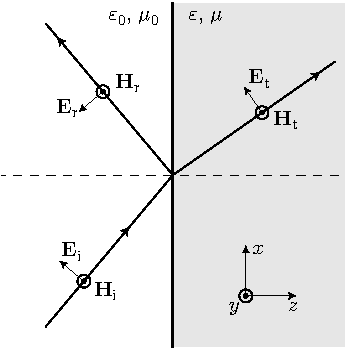
\includegraphics[width=0.4\textwidth]{fig/analytical/kvectorTM}
  \caption[Scalar polarizations at planar interface]{Scalar polarizations for EM field at a planar 
    dielectric interface.}
  \label{fig:planar}
\end{figure}

% From Maxwell's equations the electric and magnetic fields can be split into two sets: $(E_y, B_x, B_z)$
% and $(B_y,E_x,E_z)$.

% Recall that the classical action is given by 
% \begin{equation}
%   S = \frac{1}{2}\int d\vect{r}\, \big(\vect{E}\cdot\vect{D} - \vect{B}\cdot\vect{H}\big). 
% \end{equation}



\subsection{Scalar Polarization Partition Functions}

In the TE polarization the electric field is described by a single scalar field, $\vect{E}=\partial_t\phi\hat{y}$,
where  $\phi:=\phi(\vect{r},t)$.  In this case $\phi$ corresponds to the y-component of the vector potential.  
The magnetic field can also be written in terms of this scalar.
In Coulomb gauge $\nabla\cdot\vect{A}=0$, and using Maxwell's equations, the square of the magnetic
field is $|\vect{B}|^2=|\nabla\phi|^2$.
The action for the TE scalar $\phi:=\phi(\vect{r},t)$ is then given by
\begin{equation}
  S\subTE = \int_0^T dt\, \bigg( \epsr(\vect{r})\partial_t\phi^2 - \frac{1}{\mur}|\nabla\phi|^2\bigg).
\end{equation}
The partition function can be found via the same procedure 
that was used for the Dirichlet scalar, and full vector path interal.  However, we will just skip to the final
result in terms of the partition function with the Euclidean action,
\begin{equation}
  Z\subTE = \int D\phi\, \exp\left[-\frac{1}{2}\int d\vect{r} \int_0^{\beta\hbar c}d\tau
    \bigg(\epsr(\vect{r})(\partial_\tau\phi)^2 + \frac{1}{\mur(\vect{r})}|\nabla\phi|^2\bigg)\right].
\end{equation}
The field $\phi$ can be rescaled as $\tilde{\phi}:=\sqrt{\mur}\phi$ for the same reasons to the matrix path integral:  
The scaled field yields a Gaussian probability density in the worldline, 
and sidesteps any possible issues related to quantizing a field on a curved manifold.
The path integral can be rewritten in terms of these new variables, and after an integration by parts is given by
\begin{equation}
  Z\subTE = \int D\phi\, \exp\left[-\frac{1}{2}\int d\vect{r} \int_0^{\beta\hbar c}d\tau
    \,\phi\bigg(-\epsr\mur\partial^2_\tau 
    - \sqrt{\mur}\,\nabla\cdot\frac{1}{\mur}\nabla\sqrt{\mur}\bigg)\phi\right].
\end{equation}
The gradients can be expanded out in the same fashion as Eq.~(\ref{eq:TM_potential_derivatives}), which
yields an additional potential, 
\begin{equation}
  V\subTE(z) := \frac{1}{2}\big[(\partial_z\log\sqrt{\mur})^2-\partial_z^2\log\sqrt{\mur}\big].
\end{equation}
The Gaussian integral over $\phi$ can be carried out, with the result
\begin{equation}
  Z\subTE = \det\bigg(-\frac{1}{2}[\epsr(z)\mur(z)\partial_\tau^2+\nabla^2]+V\subTE(z)  \bigg)^{-1/2}.
\end{equation}

A similar derivation is possible for fields where $\vect{H}:=\partial_t\psi\hat{y}$.
In that case electromagnetic duality~(\ref{eq:EM_duality}) can be exploited to rewrite our results.
% Maxwell's equations are invariant under the following duality transformation in the absence of sources:
% $\epsr\Leftrightarrow \mu, \vect{D}\Leftrightarrow \vect{B}, \vect{E}\Leftrightarrow-\vect{H}$.
As one might expect, this field theory can be naturally formulated in terms of the dual potentials, 
subject to ``dual Coulomb gauge'', $\nabla\cdot\vect{C}=0$.
Exactly the same manipulations as the TE case can be carried out, but with $\epsr$ and $\mur$ exchanged.
The TM partition function is 
\begin{equation}
  Z\subTM = \det\bigg(-\frac{1}{2}[\epsr(z)\mur(z)\partial_\tau^2+\nabla^2]+V\subTM(z)  \bigg)^{-1/2},
\end{equation}
where the potential is 
\begin{equation}
  V\subTM(z) := \frac{1}{2}\big[(\partial_z\log\sqrt{\epsr})^2-\partial_z^2\log\sqrt{\epsr}\big].
\end{equation}
Note that the potential depends on the dielectric function in this case, and will play a much larger
role for most media.  
The simplicity of this derivation is one reason for working with both magnetic and dielectric media in this geometry.  
However, we will often set $\mur=1$, since magnetic media are rare in typical quantum optical situations.  

\subsection{TE Polarization Worldline}

It is a straightforward matter to develop the TE worldline path-integral.  In the same fashion
as the Dirichlet scalar method in Sec.~\ref{sec:dirichlet_worldline}, one uses two formal identities to rewrite the free energy in exponential form.
The renormalized TE free energy is 
\begin{align}
  \cF\subTE-\cF\subTE\sup0 &= \frac{\kB T}{2}(\log\det \op{D}\subTE -\log \det \op{D}\sup0),
\end{align}
where the partition functions $Z\subTE$ were rewritten as the functional determinant of a differential operator. 
The differential operators are 
\begin{align}
  \op{D}\subTE&:=-\frac{1}{2}[\epsr(z)\mur(z)\partial_\tau^2+\nabla^2]+V\subTE(z) \\
  \op{D}\sup0&:=-\frac{1}{2}(\partial_\tau^2+\nabla^2).
\end{align}
The vacuum operator $\op{D}\sup0$ is the same for both polarization and is determined by setting $\epsr=\mur=1$ everywhere.  
The free energy can be written using the $\log-\det$ goes to $\tr-\log$ rule~(\ref{eq:log-det}),
and the integral representation of the logarithm~(\ref{eq:integral_log}), with the result
\begin{align}
    \cF\subTE-\cF\subTE\sup0 &= \frac{\kB T}{2} \tr(\log \op{D}\subTE -\log \op{D})\\
    &= -\frac{\kB T}{2} \int_0^\infty \frac{d\cT}{\cT}\tr\big[ \exp(-\op{D}\subTE\cT) -\exp(-\op{D}\sup0\cT)\big].
\end{align}
For simplicity, we will suppress the renormalization while developing the path integral.  The renormalization 
is easily recovered by setting $\epsr=\mur=1$ everywhere, and subtracting the result.

The worldline path integrals can be developed in the usual fashion, where differential operators 
pass over to momentum operators on the auxiliary Hilbert space.  There are no problems with 
operator ordering or commutation since $\epsr(z)\mur(z)\partial_\tau^2$ is the only case of joint position and momentum operators.
After converting the operators, the TE partition function is
\begin{align}
    \cF\subTE &= \frac{\kB T}{2}\int_0^\infty\frac{d\cT}{\cT}\int d\vect{x}_0d\tau_0
    \langle \vect{x}_0,\tau_0|e^{-\epsr(\op{z})\mur(\op{z})\partial_\tau^2+\op{\vect{p}}^2]\cT/2 - V\subTE(\op{z})\cT}
    |\vect{x}_0,\tau_0\rangle.
\end{align}
Note that although the potential only varies in one dimension, it is still necessary to evaluate the trace and path integrals
over all of the dimensions.  The path integral can be developed in the usual fashion, with one minor difference.
Since the exponential operator is independent of $\tau$, it is not necessary to develop the path integral
in the $\tau$-direction.  As a result, only single integrals over $\tau$ and $p_\tau$ will be required.
 However, it is still essential to develop the spatial path integral since $\epsr(z)\mur(z)$ and $\op{\vect{p}}^2$
do not commute.
After splitting the operator 
into the product of many terms and inserting the momentum identities, the free energy is
\begin{align}
    \cF\subTE &= -\frac{\kB T}{2}\int_0^\infty\frac{d\cT}{\cT}\int d\vect{x}_N\frac{d\tau_0 dp_\tau}{2\pi}
    \int \prod_{k=0}^{N-1}\frac{d\vect{x}_kd\vect{p}_k}{(2\pi)^{D-1}}
    \delta(\vect{x}_N-\vect{x}_0)\nonumber\\
    &\times\bigg(\prod_{j=0}^{N-1}e^{-\epsr(z_j)\mur(z_j)p_{\tau}^2\Delta\cT/2}
     e^{-\vect{p}_j^2\Delta \cT/2 +i\vect{p}_j\cdot(\vect{x}_{j+1}-\vect{x}_j)- V\subTE(z_j)\Delta\cT}
    \bigg),
\end{align}
where $\Delta\cT:=\cT/N$, and the $\delta$-functions ensure path-closure. 
The Gaussian spatial momentum integrals can be evaluated, 
and the $\tau$ integrals can be evaluated at zero temperature using
\begin{equation}
  \int_{0}^{\beta\hbar c} d\tau \int_{-\infty}^{\infty} \frac{dp_\tau }{2\pi}
  \exp\bigg(-\sum_{j=0}^N\epsr(z_j)\mur(z_j)p_{\tau}^2\frac{\Delta\cT}{2}\bigg)
= \frac{\beta\hbar c }{\sqrt{2\pi\cT\langle\epsr\mur\rangle}},
\end{equation}
where the path-average is defined as
\begin{equation}
  \langle\epsr(z)\mur(z)\rangle = \frac{1}{N}\sum_{j=0}^{N-1} \epsr(z_j)\mur(z_j) 
  = \frac{1}{\cT}\int_0^\cT dt\, \epsr[z(t)]\mur[z(t)].
\end{equation}
We will use the single angle-brackets to denote the path-average of a quantity around a particular path.  
The resulting free energy is 
\begin{align}
    \cF\subTE &= -\frac{\kB T}{2}\int_0^\infty\frac{d\cT}{\cT}\int d\vect{x}_N\int d\tau_0
    \int \prod_{k=0}^{N-1}d\vect{x}_k
    \delta(\vect{x}_N-\vect{x}_0)\frac{1}{\sqrt{2\pi\langle \epsr(z)\mur(z)\rangle\cT}}\nonumber\\
    &\times\bigg[\prod_{j=0}^{N-1}\frac{1}{(2\pi\Delta\cT)^{(D-1)/2}}
    \exp\left(-\frac{(\vect{x}_{j+1}-\vect{x}_j)^2}{2\Delta\cT} - V\subTE(z_j)\Delta\cT\right)
    \bigg].
\end{align}

% This can be further simplified by carrying out the Gaussian integrals in $\tau$, since those 
% terms carry the only $\tau$-dependence.
After carrying out the $\tau$-integrals, and enforcing $\tau_N=\tau_0$, the path integral is 
\begin{align}
    \cF\subTE &= -\frac{\kB T}{2}\int_0^\infty\frac{d\cT}{\cT}\int d\vect{x}_N\int d\tau_0
    \int \prod_{k=0}^{N-1}d\vect{x}_k
    \delta(\vect{x}_N-\vect{x}_0)\frac{1}{\sqrt{2\pi\langle \epsr(z)\mur(z)\rangle\cT}}\nonumber\\
    &\times\bigg[\prod_{j=0}^{N-1}\frac{1}{(2\pi\Delta\cT)^{(D-1)/2}}
    \exp\left(-\frac{(\vect{x}_{j+1}-\vect{x}_j)^2}{2\Delta\cT} - V\subTE(z_j)\Delta\cT\right)
    \bigg].
\end{align}
We want to use the spatial Gaussians as the probability distribution for paths, where $\vect{x}_0$ is the 
starting (and finishing) point.  
% We will need the following Gaussian integral
% \begin{align}
%   \int_{-\infty}^\infty dy\, \frac{e^{-(x-y)^2/(2\sigma_1^2)}}{\sqrt{2\pi\sigma_1^2}}\frac{e^{-(y-z)^2/(2\sigma_2^2)}}{\sqrt{2\pi\sigma_2^2}}
%       = \frac{1}{\sqrt{2\pi(\sigma_1^2+\sigma_2^2)}}e^{-(x-z)^2/[2(\sigma_1^2+\sigma_2^2)]}.
% \end{align}
% The integral shows the fact after convolving two Gaussians together, the variance of the resulting Gaussian
% is the sum of the initial Gaussians.  This is useful since the Gaussian integrals have exactly this structure.
% So after carrying out all of integrals over $\tau_1,\tau_2,\ldots,\tau_{N-1}$, the 
% result is
% \begin{align}
%   &\int \prod_{j=1}^{N-1}d\vect{x}_k \prod_{j=0}^{N}\frac{1}{\sqrt{2\pi\sigma_j^2\Delta\cT}}
%   \exp\left(-\frac{(\vect{x}_{j+1}-\vect{x}_j)^2}{2\sigma_j^2\Delta\cT}\right)\nonumber\\
%   &=\frac{1}{(2\pi\langle \sigma^2\rangle\cT)^{(D-1)/2}}
%   \exp\left(-\frac{(\vect{x}_{N}-\vect{x}_0)^2}{2\langle\sigma^2\rangle\cT}\right),\label{eq:tau-integral}
% \end{align}
The normalized Gaussian probability density is 
% The same reasoning as Eq.~(\ref{eq:tau-integral}) can be used to find the normalization for the Gaussian probability density,
% which is defined as
\begin{align}
  P(\vect{x}_1,\ldots,\vect{x}_N):=&\cN\int \prod_{j=0}^{N}\frac{1}{(2\pi\Delta\cT)^{(D-1)/2}}
  \exp\bigg(-\frac{(\vect{x}_{j+1}-\vect{x}_j)^2}{2\Delta\cT}\bigg).
\end{align}
The normalization constant $\cN$ is determined by requiring that the probability density is normalized to one,
\begin{align}
1&=\int\prod_{j=1}^{N-1} d\vect{x}_k P
\implies \cN=\left[\frac{1}{\sqrt{2\pi\cT}}\exp\left(-\frac{(\vect{x}_{N}-\vect{x}_0)^2}{2\cT}\right)\right]^{-1}.
\label{eq:Gaussian_normalization}
\end{align}

The path integral can be written as an ensemble average over closed Brownian bridges,
\begin{align}
    \cF\subTE-\cF\sup0 &= -\frac{\hbar c}{2}\int_0^\infty\frac{d\cT}{(2\pi\cT)^{D/2}\cT}\int d\vect{x}_0
    \biggdlangle
    \frac{e^{-\langle V\subTE(z)\rangle\cT}}{\sqrt{\langle \epsr(z)\mur(z)\rangle}} -1
    \biggdrangle_{\vect{x}(t)}.\label{eq:TE_worldline}
\end{align}
%where we also used $\int d\tau_0 = \beta\hbar c$ to write the free energy as the zero-temperature energy. 
For completeness we note that the corresponding TM worldline method is derived in exactly the same way, with
$V\subTM$ replacing $V\subTE$.
% the result
% \begin{align}
%     \cF\subTM-\cF\sup0 &= -\frac{\hbar c}{2}\int_0^\infty\frac{d\cT}{(2\pi\cT)^{D/2}\cT}\int d\vect{x}_0
%     \biggdlangle
%     \frac{1}{\sqrt{\langle \epsr(z)\mur(z)\rangle}} e^{-\langle V\subTM(z)\rangle\cT}-1
%     \biggdrangle_{\vect{x}(t)}.\label{eq:TM_worldline}
% \end{align}
The main difference between the two path integrals is that $V\subTE$ depends on the magnetic response, while $V\subTM$ 
depends on the dielectric response.  As a result the TM potential is much more important for typical
materials.  

Let us contrast the TE worldline (\ref{eq:TE_worldline}) with the Dirichlet worldline path integral (\ref{eq:scalar_worldline}). 
First, there is a factor $\epsr\mur$ (corresponding to the square of the refractive index) 
modifying the thermal direction and an additional potential deriving from the discontinuities of the media.
The potentials will naturally enforce boundary conditions at surfaces in certain limits, far more naturally than the 

Second, the TE path integral is adapted to a planar geometry, whereas the Dirichlet path integral is geometry
independent.  We can test this path integral in this geometry to verify that
known electromagnetic results can be recovered from this worldline formalism.  In addition we can develop 
techniques that will be useful in a general geometry, and evaluate the path integrals in a manner that should straightforwardly
generalize.  We will see that this path integral can recover the Dirichlet results in the strong-coupling
$\epsr\rightarrow\infty$ limit.  So despite being adapted to a particular geometry
the TE path integral may suggest ways to develop a better uncontrolled approximation to the full path integral.

This derivation assumed zero temperature throughout, or the $\beta\rightarrow\infty$ limit. 
An alternative, more careful approach does not even develop the path integral in $\tau$, since the only 
dependence in that direction is carried by $\op{p}_\tau$.   It is essential to develop the spatial
path integral, since the prefactors of this term do not commute with the spatial momentum operators.  
The better derivation works with the Matsubara frequencies.  In the above working replace $\op{p}_\tau$ with $s_n$,
where each separate Matsubara frequency contributes separately.  At the end of the calculation the zero-temperature
limit can be taken to convert the sum over Matsubara frequencies into an integral.  The integral over the frequency
yields the answer quoted above.  

\section{Nonzero temperature Worldline Path Integrals}

It has been found that the correct dispersion dependent results can be found by the simple 
substitution $\epsr(\vect{r})\rightarrow\epsr(\vect{r},i\omega)$.  This was carefully examined 
in the context of the Lifshitz theory by Barush and Ginzburg~\cite{Barash1975}, and more recently
Rosa\etal\cite{Rosa2010}.  As noted earlier, Rahi\etal derived their effective Lagrangian at finite
temperature via linear-response theory~\cite{Rahi2009}.  Presumably the same arguments apply here 
%   Then   
% \begin{equation}
%   Z\subTE = \int D\phi \exp\left[ -\frac{\epsilon_0 c^2 }{2 \hbar c}\int_0^\beta d\tau'\int d^3\vect{r}\, 
%     \left( \epsr(\vect{r})(\partial_{\tau}\phi)^2 + \frac{1}{\mur(\vect{r})}|\nabla\phi|^2\right)\right].
% \end{equation}
% \begin{shaded}
% \comment{See Dec 2012 notes for how to handle the variable counting from doubling the number of variables}
% I'm just trying to figure out the factors of 2 here - just think of the transform to Matsubara 
% frequencies as a ordinary change of variables.
%   In December I had completely reduced the problem to a discrete problem in $\beta$ as well.
%   Say I have $N_\beta$ initial time-steps.
%   I have $N_\beta$ real variables.
%   If I introduce a Fourier series, then I now have $N-2$ complex variables for $0<n<N_\beta/2$, and 2 real variables at $n=0, N_\beta/2$.
%   Furthermore we know that $\phi_n^* = \phi_{-n}$.
%   So from the Gaussian structure of the integrals over $\phi_n$, each of these $(N-2)$ integrals over $\phi_n$ is equal.
%   When I carry out the integrals I have 
% \begin{equation}
% \prod_{n=-N_\beta/2}^{N_\beta/2-1}\int D\phi_n e^{-A_n|\phi_n|^2} 
% = C\left( \frac{1}{\sqrt{A_0}}\frac{1}{\sqrt{A_{N_\beta/2}}}\prod_{n>0}\frac{1}{A_n}\right),
% \end{equation}
% where I have used 
% \begin{equation}
% \int D\phi_nD\phi_n^* e^{-A_n|\phi_n|^2} = \int D\phi_r D\phi_ie^{-A_n(\phi_r^2+\phi_n^2)} = \frac{1}{A_n}, 
% \end{equation}
% where $\phi_n = \phi_r + i \phi_i$.
%   We then consider the limit where $N_\beta\rightarrow \infty$.  
% \end{shaded}
so assume that the appropriate frequency-dependent, non-zero temperature path integral is 
\begin{equation}
Z\subTE = \prod_{n=-\infty}^{\infty} \int D\phi_n\exp\left[ -\frac{\beta \epsilon_0 c^2 }{2}
  \int d\vect{r}\, \phi_n^*(\vect{r})\left(\epsr(\vect{r},is_n)\frac{s_n^2}{c^2} 
    -\nabla\cdot\frac{1}{\mur(\vect{r},is_n)}\nabla\right)\phi_n(\vect{r})\right] .
\end{equation}
Since the path integral is periodic (since the partition function started as a trace, implying the starting and ending states 
are identical), the fields can be expanded 
in a Fourier series,
\begin{equation}
  \phi(\tau,\vect{r}) = \sum_{n=-\infty}^{\infty}e^{is_n \tau/c} \phi_n(\vect{r}).
\end{equation}
Here the Matsubara frequencies are defined as $s_n:=2\pi n/(\beta\hbar)$, and
the $\phi_n$ are complex fields.  We will also need to use the orthogonality relation,
\begin{equation}
\int_0^{\beta \hbar c}d\tau e^{i\frac{(s_n+s_m)}{c}\tau} = \beta\hbar c \delta_{n,-m},
\end{equation}
where $\phi_n^* = \phi_{-n}$ since the fields are real. 




%Now let's \comment{assume} we just handle dispersion by taking $\epsilon(\vect{r})\rightarrow \epsilon(is_n,\vect{r})$.
The same field rescalings can be carried out as for the frequency independent case.  
The Gaussian integrals for each $\phi_n$ can be carried out, so that the free energy can be written
as
\begin{equation}
-\kB T\log Z\subTE = -{\sum_{n=0}^\infty}'\log\det\left(
\epsr(is_n,\vect{\vect{r}})\mur(is_n,\vect{\vect{r}})\frac{s_n^2}{2c^2} -\frac{1}{2}\nabla^2+V\subTE^{(n)}\right),
\end{equation}
where prime on the sum indicates that the $n=0$ is multiplied by a half and
\begin{equation}
  V^{(n)}\subTE(z) := \frac{1}{2}\big[\big(\partial_z\log\sqrt{\mur(z,is_n)}\big)^2-\partial_z^2\log\sqrt{\mur(z,is_n)}\big].
\end{equation}
The free energy is renormalized by subtracting off the vacuum energy where $\epsr=\mur=1$ and $V\subTE^{(n)}$ is zero. 
% \begin{equation}
% \log Z\subTE -\log Z_0= -{\sum_{n=0}^\infty}'\left\{\log\det\left[ 
% \frac{1}{2}\left(\epsilon(is_n,\vect{\vect{r}})\frac{s_n^2}{c^2} -\nabla^2\right)\right] 
% - \log\det\left[ \frac{1}{2}\left(\frac{s_n^2}{c^2} -\nabla^2\right)\right]\right\}
% \end{equation}
Note that the zero frequency contribution vanishes if $\lim_{\omega\rightarrow 0}\omega^2\epsr(\omega)=0$, 
and $\mur=1$.  This is related to the dispute over the role of the zero frequency pole in the dielectric
response of a metal.  

% for $n=0$ the Matsubara frequency $s_n=0$, so we have 
% \begin{align}
%   \log\det\left[ \frac{1}{2}\left(\epsilon(0,\vect{\vect{r}})\frac{s_0^2}{c^2} -\nabla^2\right)\right]
%  - \log\det\left[ \frac{1}{2}\left(\frac{s_0^2}{c^2} -\nabla^2\right)\right] = 0.
% \end{align}
% This assumes that $\epsilon(\omega)$ has at most a simple pole at zero frequency, 
% such that $\lim_{\omega\rightarrow 0}\omega^2\epsilon(\omega)=0.$    

The nonzero temperature TE worldline path integral can be developed as before.  In this case only
a $(D-1)$-dimensional Hilbert space is needed to evaluate the trace, since the thermal dimension is 
handled with the Matsubara frequencies.
\begin{align}
\cF-\cF_0 %& = -k_BT \log \frac{Z\subTE}{Z_0} \\
% & = k_B T \frac{1}{2}{\sum_{n}}'\tr\left\{ \log\left[ \frac{1}{2}
%     \left(\epsilon(is_n,\vect{x})\frac{s_n^2}{c^2} -\nabla^2\right)\right]
% -\log\left[ \frac{1}{2}\left(\frac{s_n^2}{c^2} -\nabla^2\right)\right]\right\}\\
=&-\frac{k_BT}{2}{\sum_{n=0}^\infty}'\int_0^\infty \frac{d\cT}{\cT(2\pi \cT)^{(D-1)/2}}\int d^{D-1}x_0\,\nonumber\\
&\times\dlangle e^{-s_n^2\cT /(2c^2)} -  e^{-s_n^2\langle\epsr(\vect{x},is_n)\mur(\vect{x},is_n)\rangle\cT /(2c^2)}
e^{-\cT\langle V\subTE^{(n)}(\vect{x})\rangle}\drangle,
\label{eq:TEworldline_partition_function}
\end{align}
where the paths are $D-1$ dimensional spatial paths.  
% where we introduced the path integral.
%   In this case the operator $ e^{T\nabla^2}$ only needs a 3-dimensional Hilbert space.
%   So we also only use the normalization for 3D.
This scaling with $\cT$ also reflects the different scaling behaviors in the near-field, 
thermal and far-field regions, as these will each have different approximations to the Matsubara sum.  

The zero-temperature limit can be recovered by converting the Matsubara sum into a frequency integral.
In the limit $T\rightarrow 0$, the spacing between frequencies $\Delta s = (2\pi n)/\beta \hbar\rightarrow 0$.
If we treat the material responses as being frequency independent, then the integral over frequency
is Gaussian, and the zero temperature worldline (\ref{eq:TE_worldline}) is recovered.

% The nonzero temperature path integral is also a more natural fit for the analytical techniques we will
% employ in the next chapter.  


% \section{Quantization with Harmonic Medium and Linear Response}

% In this section we will attempt to carry out the full quantization procedure for a harmonic
% medium.  We will start from a gauge-invariant Lagrangian for the EM field coupled
% to a medium. 
% We will derive the Hamiltonian, and then compute the partition function.
%  We will then gauge-fix, and integrate out the harmonic medium.  This is essentially
% based on the approach of deriving the dielectric via linear response theory advocated in Rosa~\etal\cite{Rosa2008}.
% We will integrate out the matter-fields, and treat the interaction out to second order in the interaction.  
% We will then carry out the remaining integral over the fields.  

% This method should be well-defined perturbation theory, and follow the usual physical reasoning.  This
% should avoid any of the strange features of trying to quantize the field while it is already
% interacting with an effective medium.  

% The combined field-matter Lagrangian for the EM field interacting with a charged scalar field is
% \begin{align}
%   L =& \int d^3\vect{x}\,\bigg[ \frac{\epsilon_0}{2}(\nabla A_0+\partial_t\vect{A})^2
%   - \frac{1}{2\mu_0}(\nabla\times\vect{A})^2\nonumber\\
% &+\bigg(\partial_t+i\frac{e}{c}A_0\bigg)\phi^*\bigg(\partial_t-i\frac{e}{c}A_0\bigg)\phi
% - \bigg(\nabla+i\frac{e}{c}\vect{A}\bigg)\phi^*\bigg(\nabla-i\frac{e}{c}\vect{A}\bigg)\phi
% -\phi^*(u(x)+m^2)\phi\bigg],
% \end{align}
% where there is a potential $u(x)$ binding the charged scalar to exist only in certain regions.  We
% will take $u(x)=0$ inside the bodies, and $u(x)\rightarrow\infty$ outside the bodies.  
% The action is invariant under the combined gauge transformations,
% \begin{align}
%  A_0&\rightarrow A_0-\partial_t\alpha\\
% \vect{A} & \rightarrow \vect{A}+\nabla\alpha\\
% \phi &\rightarrow e^{-i\frac{e}{c}\alpha}\phi.
% \end{align}

% The canonical momenta are found to be
% \begin{align}
%   \pi_0 &:= \frac{\delta L}{\delta (\partial_t A_0)} = 0\\
%   \vect{\Pi} & := \frac{\delta L}{\delta(\partial_t\vect{A})} = \epsilon_0(\nabla A_0+\partial_t\vect{A})\\
%   \vect{\pi} & := \frac{\delta L}{\delta(\partial_t\phi)} = \bigg(\partial_t+i\frac{e}{c}A_0\bigg)\phi^*.
% \end{align}
% As noted before, the vanishing of $\pi_0$ is a constraint which must be maintained by the dynamics.
% Preserving this constraint will require that $\partial_t\vect{\Pi}=\nabla\cdot\vect{\Pi}=0$.
% We will employ the Gupta-Bleuler quantization, which restricts the allowed states. 

% The full Hamiltonian is 
% \begin{align}
%   H &:= \int d\vect{x}(\pi_0 \partial_t A_0+\vect{\Pi}\cdot\partial_t\vect{A}+\pi\partial_t\phi 
%   +\pi^*\partial_t\phi^*) - L\\
% %   &:= \int d\vect{x}\bigg[\vect{\Pi}\cdot\frac{(\Pi-\nabla A_0)}{\epsilon_0}
% %   +\pi(\pi^*+i\frac{e}{c}A_0\phi^*) +\pi^*(\pi-i\frac{e}{c}A_0\phi^) \\
% %  &-\frac{\vect{\Pi}^2}{2\epsilon_0} + \frac{1}{2\mu_0}(\nabla\times\vect{A})^2\nonumber\\
% % &-\frac{\pi^*\pi}{2}+ \bigg(\nabla+i\frac{e}{c}\vect{A}\bigg)\phi^*\bigg(\nabla-i\frac{e}{c}\vect{A}\bigg)\phi
% % +\phi^*(u(x)+m^2)\phi\\
%   &:= \int d\vect{x}\bigg[\frac{\vect{\Pi}^2}{2\epsilon_0}+\frac{1}{2\mu_0}(\nabla\times\vect{A})^2+\pi^*\pi 
%  +\phi^*(-\nabla^2 + u(x)+m^2)\phi\nonumber\\
%  &\hspace{1cm}  +i\frac{e}{c}A_0(\pi \phi^*-\pi^*\phi) 
%    +i\frac{e}{c}\vect{A}\cdot \big(\phi\nabla\phi^*-\phi^*\nabla\phi\big)+\frac{e^2}{c^2}|\vect{A}|^2\phi^*\phi
% +A_0\frac{\nabla\cdot\vect{\Pi}}{\epsilon_0}
%  \bigg]
% \end{align}

% Given the Hamiltonian, the partition function can be readily computed, given the Gaussian
% nature of the integrals.  The long-and-short of this procedure should be that we will find 
% $Z\sim\int D()e^{-S_E}.$
% \begin{align}
%   Z &= \tr[e^{-\beta \op{H}}]\\
%   &= \int d^2\phi d\vect{A} dA_0 \langle A_0,\vect{A}| e^{-\beta \op{H}}|A_0,\vect{A}\rangle\\
%   &= \int D\phi^*D\phi D\vect{A} DA_0 D\pi^*D\pi D\vect{\Pi}D\Pi_0\delta(\pi_0)\delta(\nabla\cdot\Pi)
%   e^{-\Delta \beta H_n +\frac{i}{\hbar}(\vect{\Pi}\cdot\partial_\beta \vect{A}+\pi^*\partial_\beta\phi )}
% \end{align}
% \comment{should probably split $\phi = \phi_1+i\phi_2$ integrating over complex fields requires some
% care with the book-keeping.  Then find $\pi_1,\pi_2$.  Can use $\langle \phi_1|\pi_1\rangle = e^{i\phi_1\pi_1/\hbar}$.
% }

% End result of careful integration over two independent real fields for matter, we can just skip to 
% \begin{align}
%   Z = \int D\phi^*D\phi D\vect{A}DA_0 e^{-S_E},
% \end{align}
% where
% \begin{align}
%   S_E =& \int_0^{\hbar\beta} d\tau\int d^3\vect{x}\,\bigg[ \frac{\epsilon_0}{2}(\nabla A_0+\partial_\tau\vect{A})^2
%   + \frac{1}{2\mu_0}(\nabla\times\vect{A})^2\nonumber\\
%   &+\bigg(\partial_\tau+i\frac{e}{c}A_0\bigg)\phi^*\bigg(\partial_\tau-i\frac{e}{c}A_0\bigg)\phi
%   + \bigg(\nabla+i\frac{e}{c}\vect{A}\bigg)\phi^*\bigg(\nabla-i\frac{e}{c}\vect{A}\bigg)\phi
%   +\phi^*(u(x)+m^2)\phi\bigg],
% \end{align}
% and $\tau=\hbar \beta$, and we also scaled $A_0\rightarrow \hbar^{-1} A_0$.  

% Now expand the matter part out to quadratic order in the coupling.
% \begin{align}
%   S_E =& \int_0^{\hbar\beta} d\tau\int d^3\vect{x}\,\bigg[ \frac{\epsilon_0}{2}(\nabla A_0+\partial_\tau\vect{A})^2
%   + \frac{1}{2\mu_0}(\nabla\times\vect{A})^2
%   +\phi^*\big(-\partial_\tau^2-\nabla^2+u(x)+m^2\big)\phi\nonumber\\
%   &+ i\frac{e}{c}A^\mu(\phi^*\partial_\mu\phi -\phi\partial_\mu\phi^*)
%   +\frac{e^2}{c^2}A^\mu A_\mu\phi^*\phi-i\frac{e}{c}\partial_\mu A^\mu\phi^*\phi\bigg] 
% \end{align}
% where we are using the Euclidean inner product for 4-vectors.  


% \subsection{Rahi approach}
% \begin{enumerate}
%   \item Expand exponential to second order in $e$.
%     \begin{equation}
%     e^{-\int d^4x A_\mu j^\mu} \approx (1 - \int d^4x A_\mu(x)j^\mu(x) +\frac{1}{2}\int d^4x A_\mu(x) A_\nu(y)
%     j^\mu(x)j^\nu(y))
%   \end{equation}
%   \item Evaluate Gaussian integrals,
%     \begin{equation}
%       \int D\phi D\phi^* \phi^*(x)\phi(x) e^{-\int d^4x \phi^*(x)G^{-1}\phi(x)} = G(x)
%     \end{equation}
%   \item Simplify, Re-exponentiate.
%     Some people use Kubo formula.
%     By definition for linear response, with Ohm's law 
%     \begin{equation}
%       \vect{J} = \sigma \vect{E},
%     \end{equation}
%     so $\sigma = \epsilon-1$.  
%     Kubo formula for conductivity in linear response is 
%     $\sigma^{\mu\nu}(\omega) = \int dt \langle[ j^\mu(t),j^\nu(t')] e^{-i\omega t}.$
%     Quite general relationship.  $\sigma$ is susceptibility, $[j,j]$ is Green function response.  
    
%     Hopefully can do this calculation for general 


% \end{enumerate}





%%% Local Variables: 
%%% mode: latex
%%% TeX-master: "thesis_master"
%%% End: 
